
%********************************************************************************
% Core headers
%****************************************
\documentclass[11pt]{article}
\usepackage[margin=2cm, a4paper]{geometry} % Margins
\usepackage{lmodern} % Solves some font availability problems

% Paragraph formatting
\setlength{\parindent}{0em}
\setlength{\parskip}{1ex}

\usepackage[utf8]{inputenc}

\usepackage{titlesec} % Heading formatting (title, section, etc.)
\titleformat{\section}[block]{\normalfont\bfseries\Large}{\thesection.}{0.5em}{}
\titlespacing*{\section}{0em}{1ex}{-1ex}
\titlespacing*{\subsection}{0em}{1ex}{-1ex}

%********************************************************************************
% Maths
%****************************************
\usepackage{amsmath,amssymb,amsfonts} % Equations
\usepackage{bm} % apply bold to special symbols (only use on Greek letters, not normal letters)
\usepackage{commath} % derivatives, brackets
\usepackage{tensor} % left subscripts / superscripts
\usepackage{textcomp, gensymb} % Symbol: \degree

%********************************************************************************
% Images & Tables
%****************************************
\usepackage{graphicx}
\usepackage{placeins} % \FloatBarrier
\usepackage{caption} % Improvements to figures, extends functionality with more options

%********************************************************************************
% Formatted Blocks of Text
%****************************************
\usepackage{fvextra} % \Verb for code blocks
\usepackage{csquotes} % Block quotations
\usepackage{changepage} % Change margins for only a section
\usepackage[multiple]{footmisc} % Multiple comma separated footnote marks to one person

% Code blocks
% Using \verb allows underscores, single quotes, etc. but it doesn't play nice inside of other environments
\usepackage{xcolor}
\definecolor{bj-light-gray}{gray}{0.9}
\newcommand{\code}[1]{\colorbox{bj-light-gray}{\Verb{#1}}}

%********************************************************************************
% Text Modification
%****************************************
\renewcommand{\familydefault}{\sfdefault} % Change to font: sans serif
\hyphenpenalty=10000 % prevent hyphenation (Part 1/2)
\exhyphenpenalty=10000 % prevent hyphenation (Part 2/2)
\hfuzz=2.0em % Suppress warnings for \hbox overflow ("overfull \hbox") by up to given length
\hbadness=2000 % range=[0,10000] Suppress warnings for underfull \hbox up to given badness level

\usepackage[colorlinks=true, allcolors=blue]{hyperref} % Hyperlinks

%********************************************************************************
% Citations & Bibliography
%****************************************
\usepackage[style=numeric, sorting=none, isbn=false, url=true, sortcites=true]{biblatex}
\addbibresource{bib/bibliography.bib}

% Figure & table ref
\renewcommand{\figref}[1]{Fig.~\ref{#1}}
\newcommand{\tbref}[1]{Table~\ref{#1}}
\renewcommand{\secref}[1]{Section~\ref{#1}}
\renewcommand{\appref}[1]{Appendix~\ref{#1}}

%********************************************************************************
% Other
%****************************************
\usepackage{datetime2} % Display the date of pdf compilation as YYYY-MM-DD with the command "\date"

%********************************************************************************
% Command definition
%****************************************
\usepackage{xargs} % Define commands with multiple optional arguments as key values pairs

%%% Maths
% Position Vector (measure frame, point name, exponent)
\newcommandx*{\pos}[3][3={}]{
    \tensor*[^{#1}] {\mathbf{p}} {^{#3}_{#2}}
}
% Transformation Matrix (new frame, old frame)
\newcommandx*{\transformation}[3][3={}]{
    \tensor*[^{#1}_{#2}] {\mathbf{T}} {^{#3}}
}
% Frame(frame)
% NOTE: This is matched to the latex used in figure "CWM installation detailed v3"
% Using inkscape: Extensions > Render > Formula (pdflatex)
\newcommandx*{\refFrame}[1]{
    \mathcal{F}_{\text{#1}}
}


%%%%%%%%%%%%%%%%%%%%%%%%%%%%%%%%%%%%%%%%%%%%%%%%%%%%%%%%%%%%%%%%%%%%%%%%%%%%%%%%%
% Start
%%%%%%%%%%%%%%%%%%%%%%%%%%%%%%%%%%%%%%%%%
\begin{document}
% Title with double rule
%   Lengths: r1=1.6, gap=1.6, r2=0.4, txtGap=0.5\baselineskip
\begin{center}
    {\LARGE User Guide\\[0.5\baselineskip]
    \textbf{Glass Curtain Wall Installation Dataset}}\\[1\baselineskip]
    
    Brandon Johns\footnotemark[1]\footnotemark[2] \href{https://orcid.org/0000-0002-8761-5432}{
\includegraphics[height=2ex]{fig/ORCIDiD_iconvector.pdf}} $\boldsymbol{\cdot}$
    Elahe Abdi\footnotemark[1] \href{https://orcid.org/0000-0003-3748-0442}{
\includegraphics[height=2ex]{fig/ORCIDiD_iconvector.pdf}} $\boldsymbol{\cdot}$
    Mehrdad Arashpour\footnotemark[3] \href{https://orcid.org/0000-0003-4148-3160}{
\includegraphics[height=2ex]{fig/ORCIDiD_iconvector.pdf}}\\[0.3\baselineskip]
    \footnotemark[1]Department of Mechanical and Aerospace Engineering, Monash University, Victoria, Australia\\
    \footnotemark[2]Building 4.0 CRC, Caulfield East, Victoria, Australia\\
    \footnotemark[3]Department of Civil Engineering, Monash University, Victoria, Australia\\
    \href{mailto:brandon.johns@monash.edu}{brandon.johns@monash.edu},
    \href{mailto:elahe.abdi@monash.edu}{elahe.abdi@monash.edu},
    \href{mailto:mehrdad.arashpour@monash.edu}{mehrdad.arashpour@monash.edu}\\
    \rule{\textwidth}{1.6pt}\vspace*{-1\baselineskip}\vspace*{2pt} % r1, gap+r2
    \rule{\textwidth}{0.4pt}\\[0.5\baselineskip] % r2, txtGap
\end{center}

\begin{adjustwidth}{0cm}{0cm}
    \vspace*{-0.5\baselineskip}
    { \footnotesize \scshape Document Version \today }
\end{adjustwidth}

\vspace*{-0.8\baselineskip}
\begin{displayquote} \textit{
\textbf{Summary \textemdash}
    This document introduces the Glass Curtain Wall Installation Dataset. The dataset consists of images that depict a partially installed curtain wall as viewed from a near distance with the sun behind the camera; the camera calibration parameters; and the motion captured pose of the camera with respect to the partially installed wall.
} \end{displayquote}
\vspace*{-1\baselineskip}
\rule{\textwidth}{0.4pt}\vspace*{-1\baselineskip}\vspace{3.2pt} % r2, gap+r1
\rule{\textwidth}{1.6pt}

%%%%%%%%%%%%%%%%%%%%%%%%%%%%%%%%%%%%%%%%%%%%%%%%%%%%%%%%%%%%%%%%%%%%%%%%%%%%%%%%%
%%%%%%%%%%%%%%%%%%%%%%%%%%%%%%%%%%%%%%%%%%%%%%%%%%%%%%%%%%%%%%%%%%%%%%%%%%%%%%%%%
\section*{Introduction}
A unitised curtain wall is a type of exterior wall for high-rise buildings, which is comprised of prefabricated modules that hang from the building floor slabs. This dataset depicts a partially installed unitised curtain wall (\figref{fig:ExpAndCW}).

The dataset consists of
\begin{itemize}
    \item 140 images depicting a partially installed unitised curtain wall
    \item The camera calibration parameters
    \item Measurement of the pose (position and orientation) of the camera with respect to the wall
    \item Ground truth images for 60 images from the dataset, segmented as [glass, frame, other]
\end{itemize}

The dataset is primarily intended to be used in the development of systems to automatically measure the relative pose between the camera and the wall; systems to identify the location where the next curtain wall module (CWM) should be installed; and related user interfaces.


%%%%%%%%%%%%%%%%%%%%%%%%%%%%%%%%%%%%%%%%%%%%%%%%%%%%%%%%%%%%%%%%%%%%%%%%%%%%%%%%%
%%%%%%%%%%%%%%%%%%%%%%%%%%%%%%%%%%%%%%%%%%%%%%%%%%%%%%%%%%%%%%%%%%%%%%%%%%%%%%%%%
\section*{Data Acquisition}
The dataset was created with a 1:25 scale model (\figref{fig:ExpAndCW}). The CWMs were comprised of plain float glass in a mill-finish aluminium frame. The side of the glass that faces the building interior was coated with opaque black vinyl to emulate the effect of a coating that is commonly applied to architectural glass. The concrete building floors and columns were grey painted wood. It was noted that paint was more reflective than actual concrete. The hook-block was 3D printed plastic, and the hoist rope was twine. A Basler ace acA2040-55uc camera with a 6mm fixed focal length lens was used to take the images. The camera was set to be in focus when at the median distance.

\begin{figure}[t]
	\centering
	\centerline{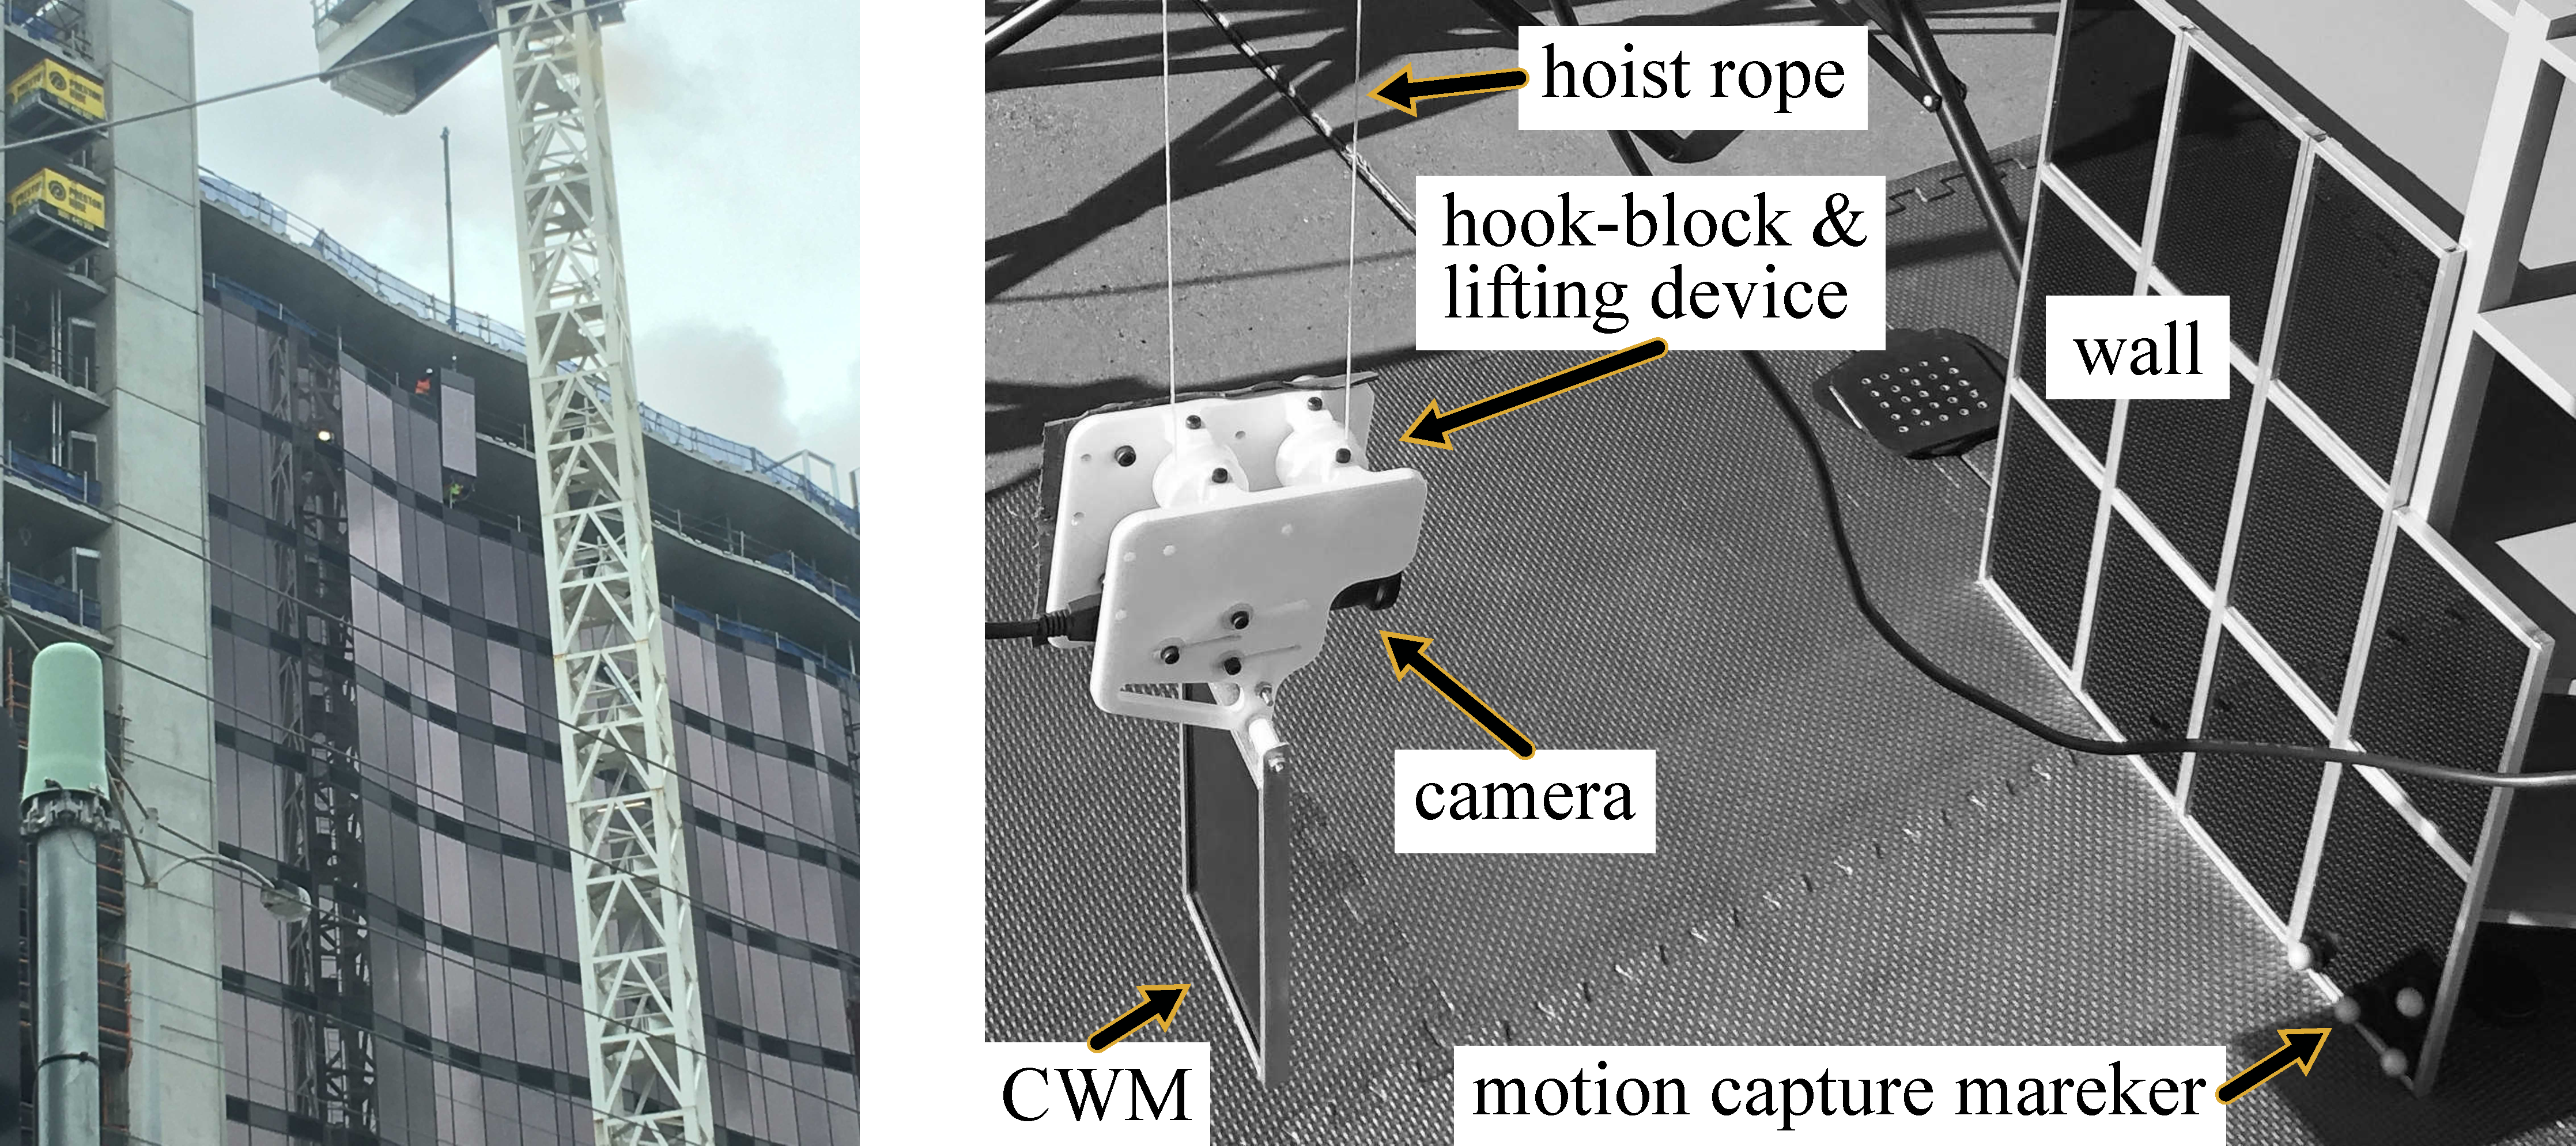
\includegraphics[width=1\columnwidth,keepaspectratio]{fig/ExperimentalSetupAndCW.pdf}}
	\caption{Left: The scenario that the dataset represents. Right: The data collection setup.}
    \label{fig:ExpAndCW}
\end{figure}

An OptiTrack motion capture system of four FLEX 13 cameras was used to locate $19$mm markers attached to the hook-block and the curtain wall. This motion capture system is not generally intended for outdoor use, hence, the accuracy of the measurements was low. The ground and the area around the markers was covered with black EVA foam mats to improve the system accuracy. Still, the majority of captured images had to be discarded due to momentary loss of tracking at the time when the image was taken. The OptiTrack system self-reported its precision as between $0.2$mm and $10$mm per object, varying with the severity of the lighting conditions.


\FloatBarrier
%%%%%%%%%%%%%%%%%%%%%%%%%%%%%%%%%%%%%%%%%%%%%%%%%%%%%%%%%%%%%%%%%%%%%%%%%%%%%%%%%
\subsection*{Calibration}
The camera calibration was performed indoors, prior to data collection. The calibration methodology follows:
\begin{enumerate}
    \item Motion capture markers were attacked to the hook block. A coordinate frame attached to these markers was defined in the motion capture software as $\refFrame{HBm}$.
    \item Motion capture markers were attached to a checkerboard. A coordinate frame attached to these markers was defined in the motion capture software as $\refFrame{CBm}$.
    \item A corner of the checkerboard pattern was assigned the coordinate frame $\refFrame{CB}$. The relative pose $\refFrame{CBm}\rightarrow\refFrame{CB}$ was measured with a ruler.
    \item The camera was used to take photos of the checkerboard whist both the camera and checkerboard were motion captured. The motion capture recorded the relative pose $\refFrame{CBm}\rightarrow\refFrame{HBm}$ at the times when each image was taken.
    \item The MATLAB Camera Calibrator was used to obtain the camera intrinsic and extrinsic parameters for these images. The calibration revealed the camera coordinate frame, which was assigned the designation $\refFrame{camera}$. The extrinsic parameters output by the calibrator described the relative pose $\refFrame{camera}\rightarrow\refFrame{CB}$, which is different for each image.
    \item The relative pose $\refFrame{HBm}\rightarrow\refFrame{camera}$ was obtained for each image through the composition of $\refFrame{HBm}\rightarrow\refFrame{CBm}\rightarrow\refFrame{CB}\rightarrow\refFrame{camera}$. The mean value of $\refFrame{HBm}\rightarrow\refFrame{camera}$ across every calibration image was taken to be the true measurement.
\end{enumerate}

To calculate the mean value of $\refFrame{HBm}\rightarrow\refFrame{camera}$, each measurement was decomposed into a $(x_i, y_i, z_i)$ translation and a $q_i$ quaternion rotation. The mean translation was then calculated as \\$(\text{mean}(x_i), \text{mean}(y_i), \text{mean}(z_i))$ and the standard deviation was calculated likewise. The mean rotation was calculated with the MATLAB Sensor Fusion and Tracking Toolbox function \code{meanrot()}, which implements the algorithm \cite{BJ4-52}. The standard deviation of the rotation was calculated as

\begin{equation}
    \sqrt{\frac{1}{n-1}\sum_{i=1}^{n}\text{dist}(q_{mean}, q_i)^2}
\end{equation}

where $n$ is the number of measurements of $\refFrame{HBm}\rightarrow\refFrame{camera}$ and the function \code{dist()} computes the angular distance between the quaternions as calculated with the MATLAB Sensor Fusion and Tracking Toolbox function \code{dist()}.

The calibrated value of $\refFrame{HBm}\rightarrow\refFrame{camera}$ for use in data collection was constructed from the mean translation and rotation. The standard deviations of the translation and rotation were $1.4$mm and $0.3\degree$ respectively.


%%%%%%%%%%%%%%%%%%%%%%%%%%%%%%%%%%%%%%%%%%%%%%%%%%%%%%%%%%%%%%%%%%%%%%%%%%%%%%%%%
\subsection*{Data Collection}
The data collection was performed according to the procedure:
\begin{enumerate}
    \item The motion capture markers attached to the hook block during calibration were left attached, and the coordinate frame $\refFrame{HBm}$ was reused.
    \item Motion capture markers were attached to a CWM on the building. A coordinate frame attached to these markers was defined in the motion capture software as $\refFrame{CWMm}$.
    \item A corner of the CWM was assigned the coordinate frame $\refFrame{wall}$. The relative pose $\refFrame{wall}\rightarrow\refFrame{CWMm}$ was measured with a ruler.
    \item The camera was used to take photos of the model whist both the camera and model were motion captured. The motion capture recorded the relative pose $\refFrame{CWMm}\rightarrow\refFrame{HBm}$ at the times when each image was taken.
    \item The relative pose $\refFrame{wall}\rightarrow\refFrame{camera}$ was obtained for each image through the composition of $\refFrame{wall}\rightarrow\refFrame{CWMm}\rightarrow\refFrame{HBm}\rightarrow\refFrame{camera}$, using the value of $\refFrame{HBm}\rightarrow\refFrame{camera}$ obtained from the calibration.
\end{enumerate}

In data collection, the camera pose, $\refFrame{wall}\rightarrow\refFrame{camera}$, was varied between $180$mm to $400$mm in distance and up to $55\degree$ in angular distance. The locations of the installed CWMs were also varied.


%%%%%%%%%%%%%%%%%%%%%%%%%%%%%%%%%%%%%%%%%%%%%%%%%%%%%%%%%%%%%%%%%%%%%%%%%%%%%%%%%
%%%%%%%%%%%%%%%%%%%%%%%%%%%%%%%%%%%%%%%%%%%%%%%%%%%%%%%%%%%%%%%%%%%%%%%%%%%%%%%%%
\section*{Data Description}
Two coordinate frames are used by the dataset (\figref{fig:ExpDimensions}). $\refFrame{camera}$ is the camera coordinate frame, resultant of the camera calibration. $\refFrame{wall}$ is the coordinate frame that is aligned with the wall.

The images are stored in the directory \code{images}, and the corresponding motion capture data in the file \code{MotionCaptureData.csv}. They correspond through the number in the filename of the image to the number in the first column of the csv. The images in directory \code{ground-truth} are manually segmented into the set [glass, frame, other] using the RGBA colour channels [blue, transparent, green]. Whilst the images in \code{images} are as-taken, the images in \code{ground-truth} have been undistorted using the camera calibration. The camera calibration parameters and the dimensions of the experimental model are described in this document, as follows.


%%%%%%%%%%%%%%%%%%%%%%%%%%%%%%%%%%%%%%%%%%%%%%%%%%%%%%%%%%%%%%%%%%%%%%%%%%%%%%%%%
\subsection*{Model Dimensions}
\begin{table}[!h]
    \centering
    \begin{tabular}{lll}
        \hline
        Description & Symbol & Value\\
        \hline
        Building floor thickness & & 9\\
        Building column cross section & & 20x20\\
        CWM frame cross section & & 10x5x1.6 channel\\
        CWM glass thickness & & 6\\
        CWM including the aluminium frame
        & $H$ & 153.2\\
        & $W$ & 103.2\\
        CWM exposed glass
        & $H_{inner}$ & 143.2\\
        & $W_{inner}$ & 93.2\\
        Height from top of panel to the next floor slab
        & $H_C$ & 129\\
        \hline
        \end{tabular}
    \caption{Dimensions of the Model. Units in mm.}
    \label{tb:ModelDimensions}
\end{table}


%\FloatBarrier
%%%%%%%%%%%%%%%%%%%%%%%%%%%%%%%%%%%%%%%%%%%%%%%%%%%%%%%%%%%%%%%%%%%%%%%%%%%%%%%%%
\subsection*{Motion Capture}
The motion capture data describes the relative pose $\refFrame{wall}\rightarrow\refFrame{camera}$, as measured in the coordinates of $\refFrame{wall}$. This is encoded as the $(x, y, z)$ position from the origin of $\refFrame{wall}$ to the origin of $\refFrame{camera}$, with units in mm, and the $(q_w, q_x, q_y, q_z)$ quaternion rotation from $\refFrame{wall}$ to $\refFrame{camera}$.

\begin{figure}[!t]
	\centering
	\centerline{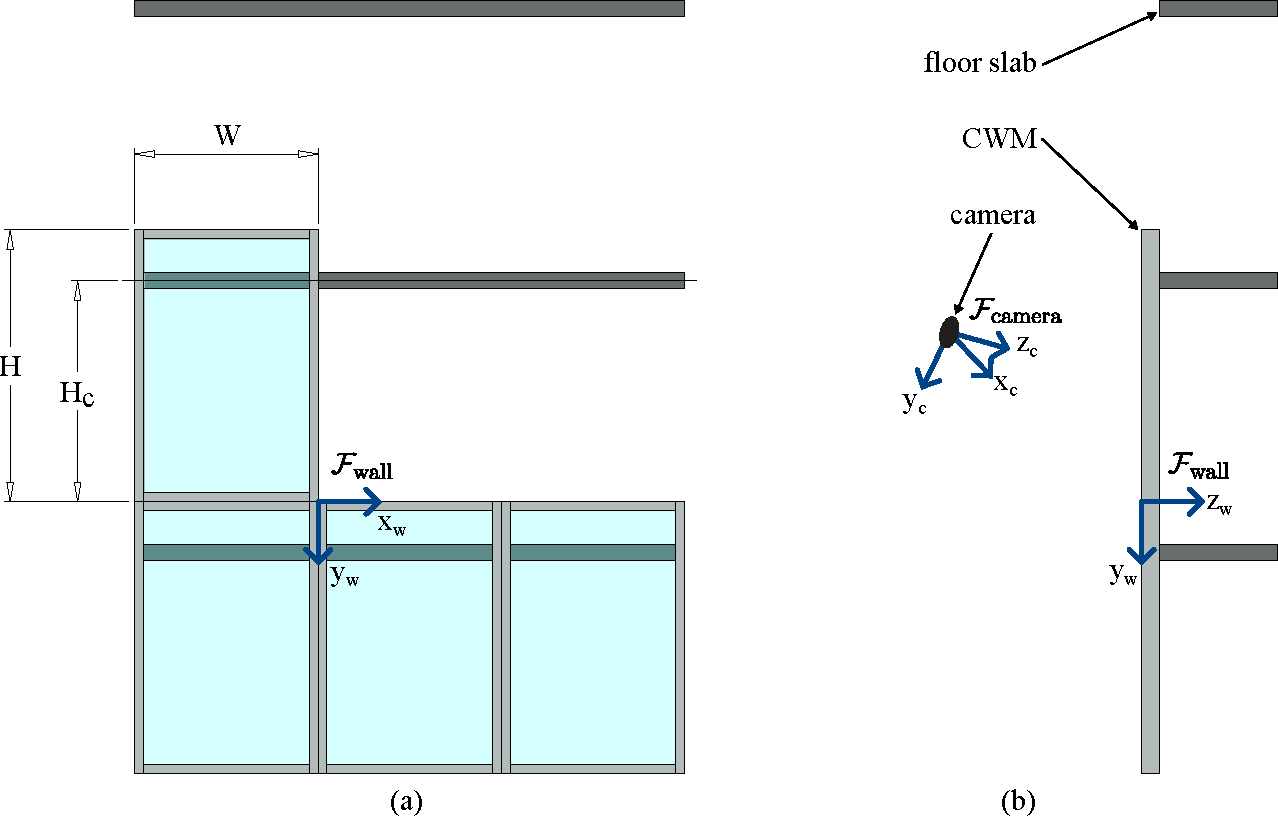
\includegraphics[width=1\columnwidth,keepaspectratio]{fig/ExpDimensions.pdf}}
	\caption{Diagram depicting the coordinate frames and model dimensions. $z_c$ points out of the camera lens, $y_c$ points down with respect to the image, and $x_c$ points horizontally with respect to the image.}
    \label{fig:ExpDimensions}
\end{figure}


%%%%%%%%%%%%%%%%%%%%%%%%%%%%%%%%%%%%%%%%%%%%%%%%%%%%%%%%%%%%%%%%%%%%%%%%%%%%%%%%%
\subsection*{Camera Parameters}
The camera intrinsic parameters resultant of the camera calibration are given in \tbref{tb:CameraParams}. The meanings and uses of these parameters are described by \cite{BJ4-53,BJ4-54,BJb-02,BJb-03} and as follows.

\begin{table}[!h]
    \centering
    \begin{tabular}{lll}
        \hline
        Description & Symbol & Value\\
        \hline
                Radial distortion coefficients
                & $k_1$ & -0.1553\\
                & $k_2$ & 0.0473\\
                & $k_3$ & 0\\
                Tangential distortion coefficients
                & $p_1$ & 0\\
                & $p_2$ & 0\\
                Focal length (px)
                & $f_x$ & 1821.0499\\
                & $f_y$ & 1817.9207\\
                Principal point (px)
                & $c_x$ & 741.8287\\
                & $c_y$ & 1019.9486\\
                Skew
                & $s$ & 0\\
                image height (px)
                & & 2048\\
                Image width (px)
                & & 1536\\
        \hline
        \end{tabular}
    \caption{Camera calibration parameters.}
    \label{tb:CameraParams}
\end{table}

Let $(X_c, Y_c, Z_c)$ be a point measured in the coordinates of $\refFrame{camera}$ with units in mm. This location is captured in the image at the pixel coordinate $(u_d,v_d)$, as measured in pixels from the top left corner of the image. The relation is described by

\begin{equation}
    \begin{bmatrix}
        u_d\\
        v_d\\
        1\\
    \end{bmatrix}
    =
    \begin{bmatrix}
        f_x & s & c_x\\
        0 & f_y & c_y\\
        0 & 0 & 1\\
    \end{bmatrix}
    \cdot
    \begin{bmatrix}
        \alpha X_c/Z_c\\
        \alpha Y_c/Z_c\\
        1\\
    \end{bmatrix}
\end{equation}

\begin{align} \label{eq:undistort}
    \alpha& = (1 + k_1r^2 + k_2r^4 + k_3r^6)\\
    r &= \sqrt{(X_c/Z_c)^2 + (Y_c/Z_c)^2}
\end{align}


%%%%%%%%%%%%%%%%%%%%%%%%%%%%%%%%%%%%%%%%%%%%%%%%%%%%%%%%%%%%%%%%%%%%%%%%%%%%%%%%%
%%%%%%%%%%%%%%%%%%%%%%%%%%%%%%%%%%%%%%%%%%%%%%%%%%%%%%%%%%%%%%%%%%%%%%%%%%%%%%%%%
\section*{Example Python / MATLAB Code}
The provided Python / MATLAB code are minimalist examples to demonstrate the relationship between the images, camera calibration, and motion capture data. The program takes a user provided point, as measured in $\refFrame{wall}$, and then plots this point on the image.

To run:
\begin{enumerate}
    \item The directory structure of this dataset should be as-downloaded
    \item Run the file \code{run_WorldToImage.py} or \code{run_WorldToImage.m}
    \item Compare the result to file \code{run_WorldToImage-ExpectedOutput.jpg}
\end{enumerate}

Information on the supporting classes can be obtained with the \code{help} command.


%%%%%%%%%%%%%%%%%%%%%%%%%%%%%%%%%%%%%%%%%%%%%%%%%%%%%%%%%%%%%%%%%%%%%%%%%%%%%%%%%
%%%%%%%%%%%%%%%%%%%%%%%%%%%%%%%%%%%%%%%%%%%%%%%%%%%%%%%%%%%%%%%%%%%%%%%%%%%%%%%%%
\section*{Acknowledgments}
This research was supported by an Australian Government Research Training Program (RTP) Scholarship. This research is supported by Building 4.0 CRC. The support of the Commonwealth of Australia through the Cooperative Research Centre Programme is acknowledged.


%%%%%%%%%%%%%%%%%%%%%%%%%%%%%%%%%%%%%%%%%%%%%%%%%%%%%%%%%%%%%%%%%%%%%%%%%%%%%%%%%
%%%%%%%%%%%%%%%%%%%%%%%%%%%%%%%%%%%%%%%%%%%%%%%%%%%%%%%%%%%%%%%%%%%%%%%%%%%%%%%%%
% References
\printbibliography


%%%%%%%%%%%%%%%%%%%%%%%%%%%%%%%%%%%%%%%%%%%%%%%%%%%%%%%%%%%%%%%%%%%%%%%%%%%%%%%%%
%%%%%%%%%%%%%%%%%%%%%%%%%%%%%%%%%%%%%%%%%%%%%%%%%%%%%%%%%%%%%%%%%%%%%%%%%%%%%%%%%
\end{document}

